\documentclass[letter]{article}
% Set target color model to RGB
\usepackage[inner=2.0cm,outer=2.0cm,top=2.5cm,bottom=2.5cm]{geometry}
\usepackage{setspace}
\usepackage[dvipsnames]{xcolor}
\usepackage{verbatim}
\usepackage{subcaption}
\usepackage{biblatex}
\usepackage{amsgen,amsmath,amstext,amsbsy,amsopn,tikz,amssymb,tkz-linknodes}
\usepackage{float}
\usepackage{fancyhdr}
\usepackage[colorlinks=true, urlcolor=blue,  linkcolor=blue, citecolor=blue]{hyperref}
\usepackage[colorinlistoftodos]{todonotes}
\usepackage{rotating}
\usepackage{booktabs}

\hypersetup{%
pdfauthor={Paul Shao},%
pdftitle={Worksheet},%
pdfkeywords={Tikz,latex,bootstrap,uncertaintes},%
pdfcreator={PDFLaTeX},%
pdfproducer={PDFLaTeX},%
}

\newcommand{\ra}[1]{\renewcommand{\arraystretch}{#1}}

\newtheorem{thm}{Theorem}[section]
\newtheorem{prop}[thm]{Proposition}
\newtheorem{lem}[thm]{Lemma}
\newtheorem{cor}[thm]{Corollary}
\newtheorem{defn}[thm]{Definition}
\newtheorem{rem}[thm]{Remark}
\numberwithin{equation}{section}

\newcommand{\homework}[5]{
   \pagestyle{myheadings}
   \thispagestyle{plain}
   \newpage
   \setcounter{page}{1}
   \noindent
   \begin{center}
   \framebox{
      \vbox{\vspace{2mm}
    \hbox to 6.28in { {\bf CSM 16A \hfill {\small #2}} }
       \vspace{6mm}
       \hbox to 6.28in { {\LARGE \hfill #1  \hfill} }
       \vspace{6mm}
       \hbox to 6.28in { {\it Term: {\rm #3} \hfill Name: \hspace{2cm}{\rm #4}}}
      \vspace{2mm}}
   }
   \end{center}
   \markboth{#5 -- #1}{#5 -- #1}
   \vspace*{4mm}
}

\newcommand{\problem}[1]{~\\\fbox{\textbf{Problem #1}}\hfill}
\newcommand{\subproblem}[1]{~\newline\textbf{(#1)}}
\newcommand{\D}{\mathcal{D}}
\newcommand{\Hy}{\mathcal{H}}
\newcommand{\VS}{\textrm{VS}}
\newcommand{\solution}{~\newline\textbf{\textit{(Solution)}} }

\newcommand{\bbF}{\mathbb{F}}
\newcommand{\bbX}{\mathbb{X}}
\newcommand{\bI}{\mathbf{I}}
\newcommand{\bX}{\mathbf{X}}
\newcommand{\bY}{\mathbf{Y}}
\newcommand{\bepsilon}{\boldsymbol{\epsilon}}
\newcommand{\balpha}{\boldsymbol{\alpha}}
\newcommand{\bbeta}{\boldsymbol{\beta}}
\newcommand{\0}{\mathbf{0}}

\newcommand{\sol}[1]{{\color{blue} \textbf{Solution: } #1}} % solutions in blue
\newcommand{\learning}[1]{{\color{ForestGreen} \textbf{Learning Goal: } #1}}
\newcommand{\note}[1]{{\color{purple} \textbf{Meta: } #1}} % notes in green
\newcommand{\answerbox}[1]{
   \noindent\fbox{
      \parbox{16cm}{
          \hspace{16cm}
          \vspace{#1}
      }
  }
}
\newcommand{\statement}[1]{
   \noindent\fbox{
      \parbox{16cm}{
          #1
      }
  }
}
\renewcommand{\answerbox}[1]{}
\begin{document}
\homework{\textbf{Week 5 Worksheet {\color{purple} Metas}}}{Designing Information Systems and Devices}{\textbf{Spring 2020}}{}{}
\problem{1: Introduction to Circuit Components}
\\
\note{
Introduction to basic circuit components.
Mentors: do a mini lecture on what is charge, what is voltage, and what is current. See lecture notes for definitions. 
}

In this problem, we will introduce the fundamental circuit components. 

\begin{enumerate}

\item{
What is a voltage source?
}

\sol{
Firstly, a voltage source is represented in this manner: 
\begin{center}
    \begin{circuitikz}
        \draw(0,0)
	    to[V=$V$] ++(1,0);
    \end{circuitikz}
\end{center}

A voltage source \textbf{guarantees} that the potential at its positive end will be $V$ more than the potential at its negative end, no matter what. 
}

\item{
 What is a current source?  
}

\sol{
A current source is represented in this manner: 
\begin{center}
    \begin{circuitikz}
        \draw(0,0)
	     to[I, l=$I$] ++(1,0);
    \end{circuitikz}
\end{center}
A current source \textbf{guarantees} that the current passing through the unit in the direction of the arrow will be its designated value. 
}

\item{What is voltage? What is a voltage drop?}

\sol{
For our discussion, it suffices to think of voltage as a kind of driver for current. Current is the movement of charges. A voltage difference forces current to move from the point (node) that has higher voltage, to the point that has lower voltage. 

Voltage drop is the voltage lost (decline of nodal voltage) across a circuit component. 
}

\item{Consider the figure below. If $V_1 \neq V_2$, what will happen to the circuit?

\begin{center}
    \begin{circuitikz}
    \draw(0,4)
	%to[short] ++(0,-1)
	to[V_=$V_1$] ++(0,-4)
	to[short] node[ground] {} ++(0,-1);
	
	\draw(0,4)
	to[short] ++(2,0)
	to[V_=$V_2$] ++(0,-4)
	to[short] ++(-2,0);
    \end{circuitikz}
\end{center}

}

\sol{
Let us designate the potential at the positive end of $V_1$ to be $V^+_1$, the potential at the negative end of $V_1$ to be $V^-_1$, the potential at the positive end of $V_2$ to be $V^+_2$, and the potential at the negative end of $V_2$ to be $V^-_2$. $V^-_1$ and $V^-_2$ are equal to 0 because of the ground. Then, the potential across $V_1$ is $V^+_1$, and the potential across $V_2$ is $V^+_2$. Since $V^+_1$ and $V^+_2$ are connected by a wire, they must be the same voltage; we know that a wire does not affect a circuit's behavior, so the voltage must stay constant across it. 
This means that $V^+_1 = V^+_2$. However, we know that the voltage potential $V^+_1 - V^-_1$ is not equal to $V^+_2 - V^-_1$ as given in the question. Hence, we see that we cannot have two voltage sources connected in this configuration.
}

\item {What happens in this case if $I_1 \neq I_2$?
\begin{center}
    \begin{circuitikz}
    \draw(0,0) 
    to[I=$I_1$] ++(0,2)
    to[I=$I_2$] ++(0,2);
    \end{circuitikz}
\end{center}
}

\sol{
The current source at the bottom guarantees that through that wire there will be $I_1$ current going through, and the current source at the top guaranteed that $I_2$ current goes through that wire. This is a contradiction, and is not theoretically possible in a circuit. 

Also, look at the point in between the two current sources. $I_1$ enters on one end, and $I_2$ leaves on the other end. This is impossible.
}

\item{
What is a resistor? 
}

\sol{
A resistor is represented in this manner: 
\begin{center}
	\begin{circuitikz}

	\draw(0,0)
	to[R, v=$ $, i=$ $] ++(3,0);
	\end{circuitikz}
	\end{center}
A resistor is a circuit unit designed to `resist' the flow of current. Following convention, there is a ``voltage drop'' across a resistor from the positive end to the negative end. The voltage drop across a resistor is $V_R = I_R R$, where $V_R$ is the voltage drop, $I_R$ is the current through the resistor and $R$ is the resistance of the resistor. 
}

\item{What is power?}

\sol{
Power is the rate at which work is done, where work is in terms of electrical energy.

For circuits, the power \textit{consumed} or \textit{dissipated} by a device is $P = IV$, where the current and voltage abide by passive sign convention.

\textbf{Common Misconceptions:}
\begin{itemize}
	\item Active components do not necessarily dissipate negative power! Consider the following circuit:
	\begin{center}
		\begin{circuitikz}
			\draw
			(0,0) node[ground] () {}
				to[V=$1\si{\volt}$, invert] ++(0,2)
				to[R=$1\si{\ohm}$] ++(2,0)
			(2,0) node[ground] () {}
				to[V=$2\si{\volt}$, invert] ++(0,2);
		\end{circuitikz}
	\end{center}
	When calculating the power dissipated by the LHS voltage source, we see the current flows counterclockwise about the circuit. With passive sign convention, we calculate the power $P_{V_1} = 1\si{\volt} \times 1\si{\ampere}$, which is positive! The left-side voltage source is dissipating power.
\end{itemize}
}

\end{enumerate}
\newpage
\problem{2: Passive Sign Convention}
\\
% Lydia Lee, Spring 2019
% lydia.lee@berkeley.edu
For the following components, label all the missing $V_\text{element}$, $I_\text{element}$, and +/- signs. \textit{Hint: The value of the voltage and current sources shouldn't affect passive sign convention---remember that voltage and current can be negative!}
\begin{enumerate}

\note{For parts (a) and (b), make sure to clarify to your students that the box figure can represent any arbitrary circuit element (a resistor, a voltage source, etc.).}
\item{
\begin{center}
	\begin{circuitikz}[scale=0.75]
		\ctikzset{resistor = european}
		\draw (0,0) to[R, v=$V_\text{element}$] ++(4,0);
	\end{circuitikz}
\end{center}
}
\sol{
\begin{center}
	\begin{circuitikz}[scale=0.75]
		\ctikzset{resistor = european}
		\draw (0,0) to[R, v=$V_\text{element}$, i=$I_\text{element}$] ++(5,0);
	\end{circuitikz}
\end{center}
}

\item{
\begin{center}
	\begin{circuitikz}[scale=0.75]
		\ctikzset{resistor = european}
		\draw (0,0) to[R, i=$I_\text{element}$] ++(5,0);
	\end{circuitikz}
\end{center}
}
\sol{
\begin{center}
	\begin{circuitikz}[scale=0.75]
		\ctikzset{resistor = european}
		\draw (0,0) to[R, v=$V_\text{element}$, i=$I_\text{element}$] ++(5,0);
	\end{circuitikz}
\end{center}
}

\item{
\begin{center}
	\begin{circuitikz}[scale=0.75]
		\draw 
		(0,0) to[V, v=$V_\text{S}$, invert] ++(0,3)
			to[open] ++(.5,0)
			to[open, v^=$V_\text{element}$] ++(0,-3);
	\end{circuitikz}
\end{center}
}
\sol{
\begin{center}
	\begin{circuitikz}[scale=0.75]
		\draw 
		(0,0) to[V, v=$V_\text{S}$, i=$I_\text{element}$, invert] ++(0,3)
			to[open] ++(.5,0)
			to[open, v^=$V_\text{element}$] ++(0,-3);
	\end{circuitikz}
\end{center}
}

\item{
\begin{center}
	\begin{circuitikz}[scale=0.75]
		\draw 
		(0,0) to[V, v=$1\si{\volt}$, invert] ++(0,3)
		(0,0) to[open] ++(.5,0)
			to[open, v_=$V_\text{element}$] ++(0,3);
	\end{circuitikz}
\end{center}
}

\note{If students are confused by this answer, draw the source on the board, then a box around it. Shade in the box so the voltage source is obscured, and now the problem is identical to having a black box voltage source. This particular style of question has featured on several exams, and it's good to have lots of practice with this when calculating power.
}

\sol{
\begin{center}
	\begin{circuitikz}[scale=0.75]
		\draw 
		(0,0) to[V, v=$1\si{\volt}$, invert] ++(0,3)
		(0,0) to[open] ++(.5,0)
			to[open, v_=$V_\text{element}$] ++(0,3)
		(0,0) to[open, i=$I_\text{element}$, invert] ++(0,3);
	\end{circuitikz}
\end{center}
}

\item{ 
\begin{center}
	\begin{circuitikz}[scale=0.75]
		\draw 
		(0,0) to[V, v=$V_\text{S}$, i=$I_\text{element}$, invert] ++(0,3);
	\end{circuitikz}
\end{center}
}
\sol{
\begin{center}
	\begin{circuitikz}[scale=0.75]
		\draw 
		(0,0) to[V, v=$V_\text{S}$, i=$I_\text{element}$, invert] ++(0,3)
			to[open] ++(.5,0)
			to[open, v^=$V_\text{element}$] ++(0,-3);
	\end{circuitikz}
\end{center}
}

\newpage
\item{
\begin{center}
	\begin{circuitikz}[scale=0.75]
		\draw 
		(0,0) to[V, v=$-1\si{\volt}$, invert] ++(0,3)
		(0,0) to[open, i=$I_\text{element}$, invert] ++(0,3);
	\end{circuitikz}
\end{center}
}
\sol{
\begin{center}
	\begin{circuitikz}[scale=0.75]
		\draw 
		(0,0) to[V, v=$-1\si{\volt}$, invert] ++(0,3)
		(0,0) to[open] ++(.5,0)
			to[open, v_=$V_\text{element}$] ++(0,3)
		(0,0) to[open, i=$I_\text{element}$, invert] ++(0,3);
	\end{circuitikz}
\end{center}
}

\item{\textbf{(PRACTICE)}

\begin{center}
	\begin{circuitikz}[scale=0.75]
		\draw 
		(0,0) to[I, l=$I_\text{S}$, invert] ++(0,3)
			to[open] ++(.5,0)
			to[open, v^=$V_\text{element}$] ++(0,-3);
	\end{circuitikz}
\end{center}
}
\sol{
\begin{center}
	\begin{circuitikz}[scale=0.75]
		\draw 
		(0,0) to[I, l=$I_\text{S}$, invert] ++(0,3)
			to[open] ++(.5,0)
			to[open, v^=$V_\text{element}$] ++(0,-3)
		(0,3) to[open, i^=$I_\text{element}$] ++(0,-3);
	\end{circuitikz}
\end{center}
}

\item{\textbf{(PRACTICE)}

\begin{center}
	\begin{circuitikz}[scale=0.75]
		\draw 
		(0,0) to[I, l=$I_\text{S}$, invert] ++(0,3)
		(0,0) to[open] ++(.5,0)
			to[open, v_=$V_\text{element}$] ++(0,3);
	\end{circuitikz}
\end{center}
}
\sol{
\begin{center}
	\begin{circuitikz}[scale=0.75]
		\draw 
		(0,0) to[I, l=$I_\text{S}$, invert] ++(0,3)			
		(.5,0) to[open, v_=$V_\text{element}$] ++(0,3)
		(0,0) to[open, i^=$I_\text{element}$] ++(0,3);
	\end{circuitikz}
\end{center}
}

\item{\textbf{(PRACTICE)}

\begin{center}
	\begin{circuitikz}[scale=0.75]
		\draw 
		(0,0) to[I, l=$I_\text{S}$, invert] ++(0,3)
			to[open, i=$I_\text{element}$] ++(0,-3);
	\end{circuitikz}
\end{center}
}
\sol{
\begin{center}
	\begin{circuitikz}[scale=0.75]
		\draw 
		(0,0) to[I, l=$I_\text{S}$, invert] ++(0,3)
			to[open, i=$I_\text{element}$] ++(0,-3)
		(.5,3) to[open, v^=$V_\text{element}$] ++(0,-3);
	\end{circuitikz}
\end{center}
}

\item{\textbf{(PRACTICE)}

\begin{center}
	\begin{circuitikz}[scale=0.75]
		\draw 
		(0,0) to[I, l=$I_\text{S}$, invert] ++(0,3)
		(0,0) to[open, i=$I_\text{element}$, invert] ++(0,3);
	\end{circuitikz}
\end{center}
}
\sol{
\begin{center}
	\begin{circuitikz}[scale=0.75]
		\draw 
		(0,0) to[I, l=$I_\text{S}$, invert] ++(0,3)
		(0,0) to[open] ++(.5,0)
			to[open, v_=$V_\text{element}$] ++(0,3)
		(0,0) to[open, i=$I_\text{element}$, invert] ++(0,3);
	\end{circuitikz}
\end{center}
}

\item{\textbf{(PRACTICE)}

\begin{center}
	\begin{circuitikz}[scale=0.75]
		\draw (0,0) to[R, i=$I_\text{element}$] ++(-4,0);
	\end{circuitikz}
\end{center}
}
\sol{
\begin{center}
	\begin{circuitikz}[scale=0.75]
		\draw (0,0) to[R, v=$V_\text{element}$, i=$I_\text{element}$] ++(-4,0);
	\end{circuitikz}
\end{center}
}

\item{\textbf{(PRACTICE)}

\begin{center}
	\begin{circuitikz}[scale=0.75]
		\draw (0,0) to[R, v=$V_\text{element}$] ++(-4,0);
	\end{circuitikz}
\end{center}
}
\sol{
\begin{center}
	\begin{circuitikz}[scale=0.75]
		\draw (0,0) to[R, v=$V_\text{element}$, i=$I_\text{element}$] ++(-4,0);
	\end{circuitikz}
\end{center}
}
\end{enumerate}
\newpage
\problem{3: Voltage Divider Properties}
\\
Let's take a systematic look at the voltages across a resistor, and see how other components in the circuit can affect it.
Consider the following circuit:
\begin{center}
    \begin{circuitikz}
    \draw(0,0)
	to[V_=$V$,invert] ++(0,5)
 	to[short] ++(3,0)
	to[short] ++(0,-1)
	to[R,l=$R_1$] ++(0,-1)
	to[short] ++(0,-1)
	to[R,l=$R_2$] ++(0,-1)
	to[short] ++(0,-1)
	to[short] node[]{} ++(-3,0);
    \end{circuitikz}
\end{center}
\note{This problem is intended to give students a deeper understanding on voltage dividers and how circuits can get loaded. It would help students if mentors went over equivalences of resistors in series and in parallel.}

\begin{enumerate}
\item{
Calculate the voltage drop across $R_1$ and $R_2$ using series resistance calculations.}

\note{It is important to show students that we can simplify complicated circuits by using equivalence relationships.  Also help students understand why the current through the two resistors would be the same.}

\sol{The current out of the voltage source is given by Ohm's law:
\begin{align*}
    i &= \frac{V}{R_{eq}} \\
    i &= \frac{V}{R_1 + R_2}
\end{align*}
Again, by Ohm's law, we have that
\begin{align*}
V_{R_1} = i R_1 = V \frac{R_1}{R_1 + R_2} \\
V_{R_2} = i R_2 = V \frac{R_2}{R_1 + R_2}
\end{align*}}

\item Suppose we want to manipulate the voltage across $R_2$, but it's locked in a box with the voltage source, as denoted below. Can we use $R_1$ to manipulate $V_{R_2}$? What range of voltages can we achieve? 
\begin{center}
    \begin{circuitikz}[scale=0.8]
    \filldraw[fill=gray!40!white,draw=black] (-1,-0.5) rectangle (4,7.5);
    \draw(0,0)
	to[V_=$V$,invert] ++(0,7)
 	to[short,-o] ++(5,0)
	to[short] ++(0,-1)
	to[R,l=$R_1$] ++(0,-1)
	to[short,-o] ++(0,-1)
	to[short] ++(-2,0)
	to[short] ++(0,-1)
	to[short] ++(1,0)
	to[short,l=$V_{R_2}$,-o] ++(1,0)
	-- ++(-2,0)
	to[short] ++(0,-1)
	to[R,l=$R_2$] ++(0,-1)
	to[short] ++(0,-1)
	to[short,-o] ++(2,0)
	-- ++(-2,0)
	to[short] ++(-3,0)
	to[short] node[ground]{} ++(0,-1);
	
	\end{circuitikz}
\end{center}

\note{
This section highlights the different properties of voltage dividers and how the voltage drop across one component can be manipulated by the ratio resistors in the voltage divider. 
}

\sol{Any voltage in the range $(0, V]$! Notice from the equations above that $V_{R_2} = V \frac{R_2}{R_{Total}}$. If we increase $R_1$ indefinitely, holding $R_2$ constant, we can make the fraction arbitrarily small. Intuitively, since the same current flows through both $R_1$ and $R_2$, they have to split the total voltage of the power source, and larger resistances correspond to larger voltage drops (by Ohm's Law). If we decrease $R_1$ to $0$, $V_{R_2} = V$, so the voltage can be at most whatever is supplied by the power source. That the voltage source limits the achievable voltage in the circuit is a concept we will see again when we cover clipping in op-amps.}

\item Now let's try using our new variable voltage source to power a light bulb with resistance $R_L$, where the threshold voltage for lighting the bulb is $6 \text{V}$. Find $R_1$ and $R_2$ so that the voltage across $R_2$ is this threshold voltage; that is, $V_{R_2} \equiv V_{out} = 6 \text{V}$. Assume we have a $12 \text{V}$ voltage source.

\begin{center}
    \begin{circuitikz}[scale=0.8]
    \filldraw[fill=gray!40!white,draw=black] (-1,-0.5) rectangle (4,7.5);
    \draw(0,0)
	to[V_=$12 \text{V}$,invert] ++(0,7)
 	to[short,-o] ++(3,0)
	to[short] ++(0,-1)
	to[R,l=$R_1$] ++(0,-1)
	to[short,-o] ++(0,-1)
	to[short] ++(0,-1)
	to[short] ++(1,0)
	to[short,l=$\quad \quad V_{out} \equiv 6\text{V}$,-o] ++(1,0)
	-- ++(-2,0)
	to[short] ++(0,-1)
	to[R,l=$R_2$] ++(0,-1)
	to[short] ++(0,-1)
	to[short,-o] ++(2,0)
	-- ++(-2,0)
	to[short] ++(-3,0)
	to[short] node[ground]{} ++(0,-1);
	
 	\draw(5,3)[dashed] 
 	-- ++(2,0); 
 	\draw(7,3)
 	to[lamp,l=$R_L$] ++(0,-3);
%  	to[R,l=$R_L$] ++(0,-3);
 	\draw(7,0)[dashed]
 	-- ++(-2,0);
	\end{circuitikz}
\end{center}


\note{
Make sure to point out that the lightbulb is not connected yet and that we need to voltage drop across $R_2$ to be 6 volts.}

\sol{We want to split the voltage in half (from 12 to 6). Based on the voltage divider formula above, that means $R_1 = R_2 \equiv R$. Note that, under this condition, the voltage is evenly split regardless of what the actual resistance values are! While the current depends on actual resistance values, the voltage only depends on the ratio of resistances.}

\item Now that we found an $R_1$ and $R_2$ that seem to divide our voltage source appropriately, let's try to connect the bulb to the ends of $R_2$. Remember, the bulb has a resistance $R_L$. Calculate the voltage across $R_1$, $R_2$ and the light bulb when it is connected. Will the light bulb turn on?

\note{We see that once we add the resistor in parallel with R_2 the overall resistance decreases therefore our V_out will decrease as well.  It might help to point out this relationship using Ohm’s law: $V = IR$.  This is usually the most difficult section for students to conceptualize so make sure to be very clear in the relationships between different components in a circuit.}

\sol{Let's reapply the voltage divider formula, but now notice that the "second" resistor is $R_2 \| V_L$!. When we change the resistance in a voltage divider circuit, the voltage across that resistance changes as well. We find that $V_{R_1} = V \frac{R}{R + R \| R_L} = 12\text{V} \frac{R}{R + \frac{R R_L}{R + R_L}} = 12\text{V} \frac{R + R_L}{R+2 R_L}$. The rest of the potential drop must be across the $R_2$-$R_L$ system, so we have $V_{R_2} = V_{\text{bulb}} = 12\text{V} \left(1 - \frac{R + R_L} {R + 2 R_L}\right) = 12\text{V} \frac{R_L}{R + 2 R_L} \leq 12\text{V} \frac{R_L}{2 R_L} = 6\text{V}$. 


So the voltage \textit{decreased}, and the light bulb doesn't turn on. 


The takeaway from this is that, while it may seem like the voltage divider can make voltage sources of arbitrary voltages, the act of connecting a component actually changes the output of the voltage divider. We will later learn about a way to stop a light bulb (or other devices that use up power) from ``affecting" the circuit that supplies power by placing a ``buffer" between the two.}
\end{enumerate}
\newpage
\problem{4: Resistivity}
\\
% Author: Paul Shao
% Email: paulshaoyuqiao1@berkeley.edu
Resistivity is a \textbf{physical property} of the material that quantifies how much it opposes the flow of electric current.

Assume that in an ideal case, the cross-section and physical composition of the wire are uniform, We can find its resistivity with the equation below:

$$\rho = R \frac{A}{L}$$

Here, $\rho$ stands for the resistivity of the wire, $R$ stands for its resistance, $A$ stands for the area of the cross section of the wire, and $L$ stands for the length of the wire. Using this equation, we can also solve for the resistance of a wire:

$$R = \rho \frac{L}{A}$$
\note{When you are showing this question to the students, make sure you present the resistor configuration from the perspective of circuit design. The purpose of this question is not to simply review equivalent resistance, but also to come up with a way to optimize a certain goal during the process of schematics design.}

\textbf{Note:} Throughout the following parts of this question, we will be frequently referencing some of the following variables. In case you are confused about what these variables mean, we've included a section explaining what each variable stands for.
\begin{itemize}
    \item $A$: the cross section area of a single wire.
    \item $L$: the length of a single wire.
    \item $\rho_{cu}$: resistivity for the material copper.
    \item $\rho_{Al}$: resistivity for the material aluminum.
\end{itemize}
\begin{enumerate}
    \item Now, consider the rectangular copper wire below. Given that the cross-section of the wire is a square and has a cross section area of $A$, determine the overall resistance of the wire in terms of $\rho_{cu}$, $L$, and $A$.
    \sol{By the resistivity equation, the resistance of the wire is equal to:
    $$R = \rho_{cu}\frac{L}{A}$$
    }
    \begin{center}
            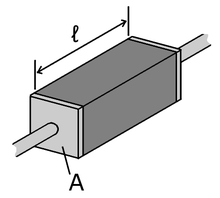
\includegraphics[scale=0.6]{../wire.png}
    \end{center}
    \item Suppose we have $N$ such wires and align them side by side to form a mega-wire. Find the overall resistance of this mega-wire. What is this configuration similar to? \\
    \note{When explaining this question to your students, make sure to show them a visual representation of the model. When drawing out the mega-wire, make sure to label the dimensions of the wire (cross-section area, length). It really helps to think visually in terms of how all the quantities that determine the resistance change.} \\
    \sol{Since we have all $N$ wires aligned side by side, we are essentially expanding the cross-section area while merging all the wires together by their lengths. This means that the new mega-wire will have a new cross-section area of $NA$ (since we are merging $N$ such wires), while its length remains the same ($L$). Hence, the overall resistance of the mega-wire will be:
    $$R_{mega} = \rho_{cu} \frac{L}{NA}$$
    }
    \item Again, with $N$ identical wires, what's a configuration that can achieve the highest resistance possible? What is this configuration similar to? \\
    \note{The question by itself might seem pretty daunting and wide in scope. However, make sure you emphasize to the students to start by applying a circuit that they are familiar with (using equivalence). The proof that the series configuration achieves the highest resistance possible shouldn't be the main focus of this question. Although providing a intuitive explanation will help the students understand the approach more.}
    \sol{The key of this question is to start from the resistance equation:
    $$R = \rho\frac{l}{A}$$
    Algebraically, we want to maximize the value of $R$ for this question. Since $\rho$ is just a physical constant, we can't really manipulate its value. Observing the fraction $\frac{l}{A}$, we can see that the overall length of the mega-wire should be as great as possible, while its cross section area should be kept as small as possible. How can we arrange $N$ wires in a way so that the overall new wire is as long as possible? \\
    We arrange in a single long line! This also helps minimize the cross section area to $A$, and we can't really go lower than that since we can't split up a wire into two (thereby splitting the cross section area). \\
    Hence, for this new mega-wire, it has a length of $NL$ and a cross section area of $A$. Applying the resistance equation, we have:
    $$R_{mega} = \rho_{cu}\frac{NL}{A}$$
    This configuration is exactly the same as a series circuit where resistors are connected in one long line. If you think in terms of the equivalent resistance for a series circuit, it also makes sense since we are summing up all the resistances.
    }
    \item Consider part (b) again, but this time, instead of $N$ copper wires, we split the number evenly between aluminum wires and copper wires. First, we have $N/2$ copper wires on the left side, and $N/2$ aluminum wires on the right side, and then we push these wires together to form a new mega-wire. What's the overall resistance of this wire? (In terms of $\rho_{cu}, \rho_{Al}, L, $ and $a$) \\
    \note{Similar to the question above, this question also emphasizes thinking from the equivalent resistance perspective. Make sure to encourage your students to think in terms of the bigger picture (overall resistance) instead of individual wires. } \\
    \sol{As we can see from part (b), when we are aligning the wires side by side, we are essentially arranging the wires to be parallel to each other. Instead of thinking in terms of individual wires, we can consider the overall mega-wire to be a mega copper wire and a mega aluminum wire in parallel! For both wires, they will have a length of $L$ and an overall cross section area of $(N/2)A$ (since we have $N/2$ wires for each category). Hence, applying the resistance equation again, we can find that:
    $$R_{cu-mega} = \rho_{cu}\frac{L}{\frac{N}{2}A} = \rho_{cu}\frac{2L}{NA}$$
    $$R_{Al-mega} = \rho_{Al}\frac{L}{\frac{N}{2}A} = \rho_{Al}\frac{2L}{NA}$$
    Now, since these 2 mega wires are parallel to each other, by equivalent resistance, we can find the overall resistance of the wire to be:
    $$R_{overall} = \frac{1}{\frac{1}{R_{cu-mega}} + \frac{1}{R_{Al-mega}}} =\left( \frac{\rho_{cu}\rho_{Al}}{\rho_{cu} + \rho_{Al}} \right)\frac{2L}{NA}$$
    If you look closely at the equation, you can actually see how the resistivities of both materials are arranged algebraically as if they are in parallel!
    }
    \item Instead of having all $N/2$ wires of \textbf{the same material} on one side before merging, now we interleave and mix every single wire together (a single copper wire can be aligned right next to a single aluminum wire), does the overall resistance of this new mega-wire change? \\
    \note{This might seem like a tricky question because there are a lot of different ways to permute all the $N$ wires. However, the key point is still on the bigger picture. Make sure to encourage the student to think in terms of equivalence (not just equivalent resistance, but also how you can actually move things around in certain circuits!)} \\
    \sol{The key to this question is to realize that, we are essentially aligning all wires in parallel, so we can rearrange all the copper wires to be together on one side and all the aluminum wires to be together on another side, and now we are back to the previous question! Hence, the overall resistance of this new mega-wire doesn't change.}
\end{enumerate}

\newpage
\problem{5: Ohm's Law}
\\
% Author: Pranshu Bansal
% Email: pranshu@berkeley.edu
\note{
Description: derive intuition behind Ohm's law and I-V plots for resistors.
}

\begin{enumerate}

\item{In the graph below, plot the equation $y = 2x + 1$.
\begin{center}
    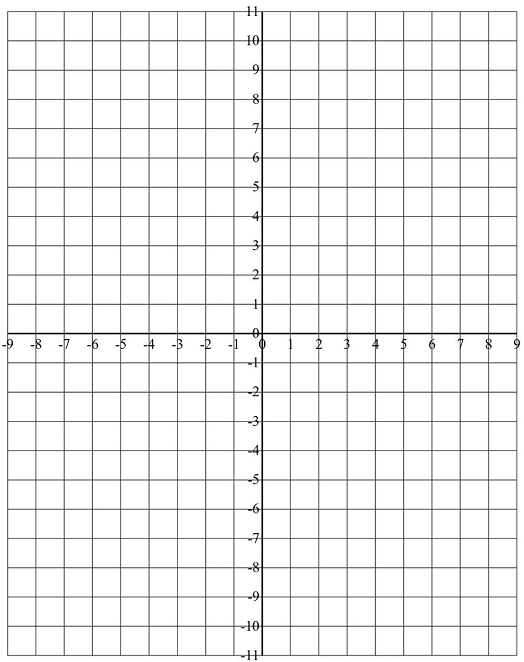
\includegraphics[scale=0.6]{../graph.png}
\end{center}
}

\sol{
\begin{center}
    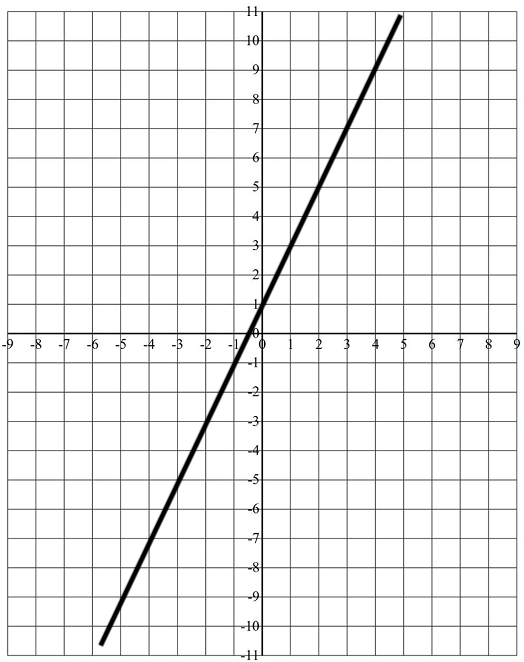
\includegraphics[scale=0.6]{../graph_sol1.png}
\end{center}
}

\item{Can this graph represent the I-V relationship of some resistor? Why or why not?}
\sol{
    No, this graph cannot represent the I-V relationship of a resistor because it doesn't pass through the origin. The current through a resistor cannot be non-zero when the voltage across it is zero and vice versa.
}

\item{Plot $y = -x$? Can it represent the I-V relationship of some resistor? Why or why not?
\begin{center}
    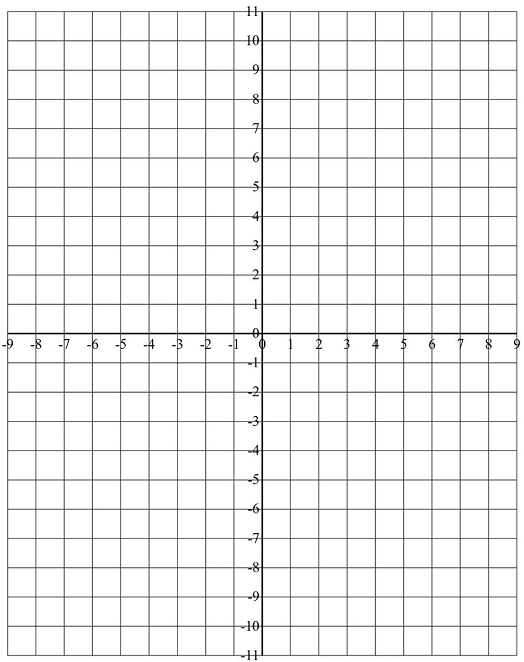
\includegraphics[scale=0.6]{../graph.png}
\end{center}
}
\sol{
\begin{center}
    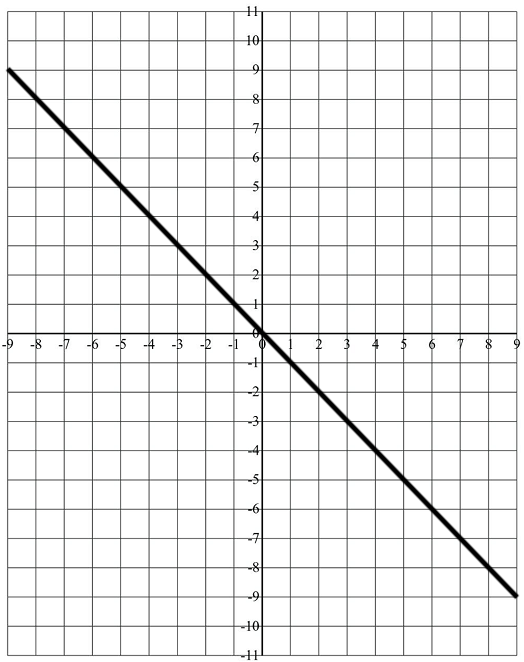
\includegraphics[scale=0.6]{../graph_sol2.png}
\end{center}
    
No. Even though this graph passes through the origin, it cannot represent the I-V relationship of a resistor because it passes through the second and fourth quadrant of the graph. The current through a resistor cannot be negative when the voltage across it is positive and vice versa.
}

\item{For a general linear equation, $y = mx + c$, what can you say about m and c for this equation to be the I-V relationship of a valid resistor?}

\sol{
For $y = mx + c$ to be a valid I-V relationship, two conditions must be satisfied. \\
The value of c has to be zero. This ensures that the current through a resistor cannot be non-zero when the voltage across it is zero and vice versa. \\
The value of m has to be positive. This ensures that the plot only passes through the first and the third quadrants. Hence, the voltage and the current always have the same sign.
}

\item{Can a non-linear polynomial be used to represent a resistor's I-V relationship?}

\sol{
    Ohm's law states that the relationship between the current through a resistor and the voltage across it is linear. Therefore, a non-linear polynomial cannot be used for such purpose.
}
\end{enumerate}

\end{document}